\section{Cost and response time}
\label{sec:cost}

\finding{\textbf{Summary.} Building a workspace costs \Nbuildlowcost{} for a low-volume
mailbox, \Nbuildmidcost{} for a mid-volume one and \Nbuildhighcost{} for a high-volume one.
Keeping it updated costs about \Nupkeeplow{}, \Nupkeepmid{} and \Nupkeephigh{} per month
respectively. The median build takes \Nlatmedian{} seconds; all \Nnbuilds{} completed builds finished in
under 30 seconds (slowest: \Nlatmax{} seconds). These are single-user figures on one provider
on one day.}

\subsection{How it was measured}
\label{sec:method}

The benchmark (\file{backend/eval/agent/bench}) runs the production flows with real model
calls against synthetic mailboxes, one run at a time, and records wall-clock time, tokens and
cost for every model call. It made \Nnruns{} runs and \Nllmcalls{} model calls for a total of
\Nbenchcost{}. A further \Nnnocredit{} runs at the very end were refused because the provider
account ran out of credits; they are excluded.

\begin{itemize}
\item \textbf{Three use cases}: online orders, supplier invoices, job applications. Each has its own prompt and its own mail.
\item \textbf{Three email volumes}, defined by how much relevant mail the last 90 days contain:
\end{itemize}

\begin{center}\small
\begin{tabularx}{0.92\linewidth}{@{}P{2.2cm}rrL@{}}
\toprule
\textbf{Volume} & \textbf{Threads to track} & \textbf{Other threads} & \textbf{Typical user} \\
\midrule
Low & 10 & 15 & A few orders or bills a month \\
Mid & 40 & 60 & Several relevant emails a week \\
High & 160 & 120 & Several a day; more than a build reads (the cap is 80 threads) \\
\bottomrule
\end{tabularx}
\end{center}

\begin{itemize}
\item \textbf{Mail that looks like real mail in size.} Threads have 1 to 3 messages. Message length is mixed: 30\% short (about 600 characters), 40\% medium (about 1,600) and 30\% long (3,200 to 4,200, above the pipeline's 3,000-character cap). Half of the ``other'' threads are promotions from the same senders, which the queries match and the agent must ignore.
\item \textbf{Three repeats} of every use case and volume (27 builds), plus builds of the eval scenarios (hand-written mailboxes of about 30 threads, each run up to twice), to widen the variety of prompts in the response-time distribution.
\item \textbf{Syncs} start from a finished build of every use case and volume and reveal 1, 3, 10 or 30 new emails: about half open new threads to track, about 30\% are follow-ups in existing threads, about 20\% are noise.
\item \textbf{Cost} is tokens multiplied by the list price of the measured model: \usd{0.45} per million input tokens and \usd{3.00} per million output tokens.
\item \textbf{Real Gmail}: the application database holds two builds, two syncs and one edit made on a real mailbox on the same day with the same configuration. Only their durations, token counts, costs and thread counts were read. They are shown next to the synthetic results as a check.
\end{itemize}

\subsection{Cost of building a workspace}

\begin{table}[H]
\centering\small
\begin{tabularx}{\linewidth}{@{}P{2.3cm}rrrrrrP{2.3cm}rP{1.6cm}@{}}
\toprule
& & \multicolumn{2}{c}{\textbf{Read}} & \multicolumn{2}{c}{\textbf{Tokens}} & \multicolumn{2}{c}{\textbf{Cost}} & \multicolumn{2}{c}{\textbf{Time}} \\
\cmidrule(lr){3-4}\cmidrule(lr){5-6}\cmidrule(lr){7-8}\cmidrule(l){9-10}
\textbf{Volume} & \textbf{n} & thr. & msg. & in & out & median & range & med. & range \\
\midrule
\tabin{generated/tab_build.tex}
\bottomrule
\end{tabularx}
\caption{Build cost and time. ``Read'' is the number of threads and messages the backfill
processed (medians). The number of threads read depends on the queries the model chooses: broad
queries also pull in threads that are then ignored.}
\label{tab:build}
\end{table}

\begin{figure}[H]
\centering
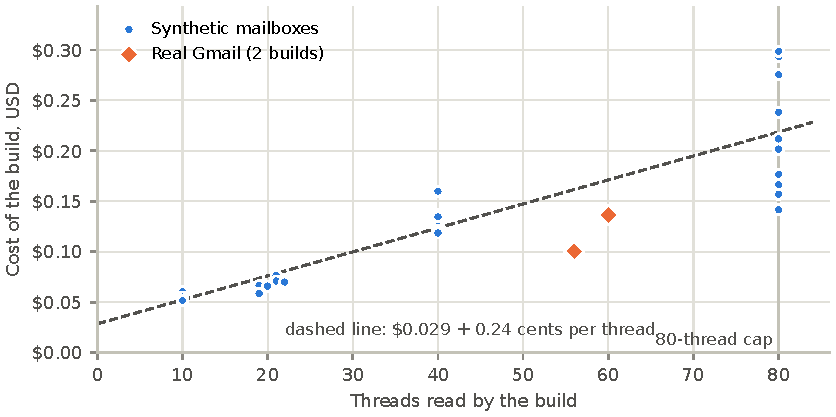
\includegraphics[width=0.86\linewidth]{figures/fig_cost_threads.pdf}
\caption{Build cost against the number of threads read. One dot per build.}
\label{fig:costthreads}
\end{figure}

Cost is close to linear in the number of threads read: a fixed part of about \Nfitfixed{}
(design and interface) plus about \Nfitperthreadcents{} cents per thread. Because a build reads
at most 80 threads, the fit puts a full build at about \Nfitcap{}. The two real Gmail builds
(56 and 60 threads, \usd{0.10} and \usd{0.14}) fall inside the synthetic cloud, which is the
main reason to trust the synthetic numbers.

\begin{figure}[H]
\centering
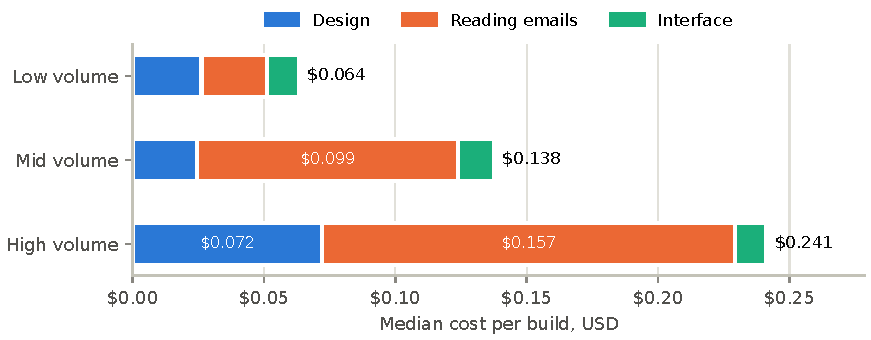
\includegraphics[width=0.86\linewidth]{figures/fig_phase_cost.pdf}
\caption{Where the money goes, by phase (median per build).}
\label{fig:phase}
\end{figure}

\begin{table}[H]
\centering\small
\begin{tabularx}{0.9\linewidth}{@{}P{1.6cm}LrLrLr@{}}
\toprule
& \multicolumn{2}{c}{\textbf{Design}} & \multicolumn{2}{c}{\textbf{Reading emails}} & \multicolumn{2}{c}{\textbf{Interface}} \\
\textbf{Volume} & cost (share) & calls & cost (share) & calls & cost (share) & calls \\
\midrule
\tabin{generated/tab_phase.tex}
\bottomrule
\end{tabularx}
\caption{Median cost and number of model calls per phase.}
\end{table}

What this means:
\begin{itemize}
\item \textbf{Design and interface are a floor} of about 4 cents per build. At low volume they are most of the bill. At high volume the design phase needed about twice as many calls (more search results to work through) and cost about 7 cents.
\item \textbf{Reading emails scales with volume} and dominates from mid volume upwards. Its cost is almost all input tokens: each batch sends the guide, the records saved so far and up to 6 threads.
\item \textbf{The worst case is bounded.} 80 threads of 10 messages at the 3,000-character cap would be far above anything measured, but a run stops at \usd{3} by configuration.
\end{itemize}

\subsection{Response time of workspace generation}

\begin{figure}[H]
\centering
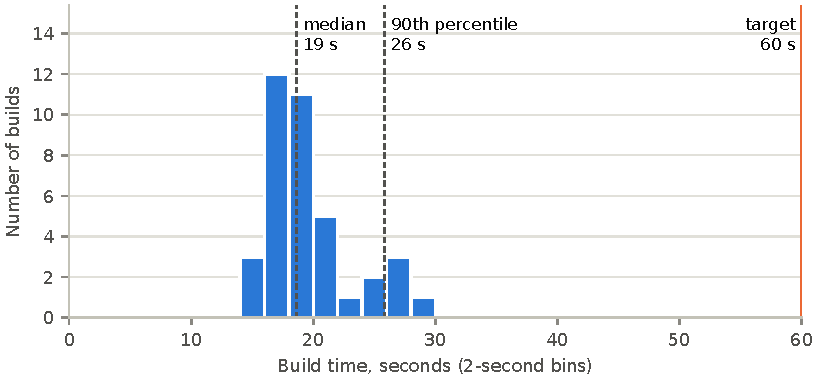
\includegraphics[width=0.86\linewidth]{figures/fig_latency_hist.pdf}
\caption{Distribution of build time over \Nnbuilds{} builds (27 on generated mailboxes, the rest
on eval scenarios), from the start of the run to the workspace being ready.}
\label{fig:lathist}
\end{figure}

\begin{table}[H]
\centering\small
\begin{tabularx}{0.86\linewidth}{@{}Lrrrrrrr@{}}
\toprule
\textbf{Builds} & \textbf{n} & \textbf{min} & \textbf{p10} & \textbf{median} & \textbf{p90} & \textbf{p95} & \textbf{max} \\
\midrule
\tabin{generated/tab_latency.tex}
\bottomrule
\end{tabularx}
\caption{Build time in seconds. Percentiles are interpolated; with these sample sizes p90 and
p95 are indicative only.}
\label{tab:latency}
\end{table}

\begin{figure}[H]
\centering
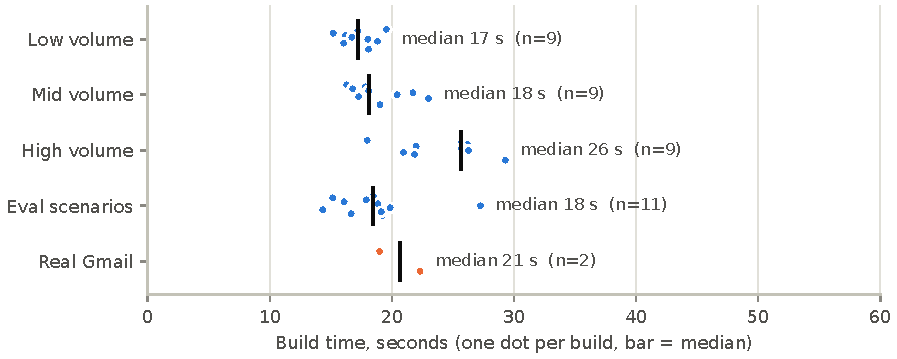
\includegraphics[width=0.86\linewidth]{figures/fig_latency_groups.pdf}
\caption{Build time by group, including the two real Gmail builds.}
\label{fig:latgroups}
\end{figure}

What this means:
\begin{itemize}
\item \textbf{Build time barely depends on email volume.} Batches are read in parallel, so 80 threads take little longer than 10. The fixed part is the design phase, which is sequential and takes about \Ndesignmedian{} seconds (about \Ndesignshare\% of a build).
\item \textbf{The target of one minute is met with margin} in this setting: all \Nnbuilds{} completed builds were under 30 seconds.
\item \textbf{What the user experiences adds up to 2 seconds of queue wait and up to 2 seconds of polling} on top of these figures, because the worker and the page both poll every 2 seconds.
\item \textbf{This distribution has no provider tail.} During the benchmark no model call had to be retried and none went to the fallback model. That is a good day, not a guarantee: each call may wait up to 60 seconds before it is retried, so on a bad provider day a build can take minutes. Earlier in the project, on other providers, builds took 199 and 398 seconds for exactly this reason.
\end{itemize}

Of the \Nnbuildsall{} builds started, \Nnbuildfail{} failed after 7 seconds: in eval scenario 07 the
model asked three times in a row to read a thread it had not found by search, and the loop
stopped the design phase. The user would see ``the agent could not finish this step'' and a
``Try again'' button. No build fell back to the built-in table view.

\subsection{Effect of the thinking pass}
\label{sec:thinking}

The model can be asked to reason before answering (\code{LLM\_REASONING\_EFFORT=low}). This
setting was not benchmarked: the provider account ran out of credits before the planned
comparison could run. The only evidence is two test builds of eval scenario 04 made with
thinking on before the benchmark, against the benchmark's builds of the same scenario with
thinking off.

\begin{table}[H]
\centering\small
\begin{tabularx}{0.8\linewidth}{@{}Lrrrr@{}}
\toprule
\textbf{Scenario 04 build} & \textbf{n} & \textbf{Time} & \textbf{Cost} & \textbf{Output tokens} \\
\midrule
Thinking off (default) & 2 & 18\,s, 19\,s & \$0.07, \$0.09 & 7.6k, 10k \\
Thinking on, low effort & 2 & 55\,s, 96\,s & \$0.12, \$0.20 & 28k, 50k \\
\bottomrule
\end{tabularx}
\caption{Thinking on and off, same scenario. Four builds: an indication, not a measurement.}
\end{table}

In the slower of the two thinking builds, three design calls produced about 16,000 output
tokens each and took 76 of the 96 seconds. Output tokens are both the expensive ones and the
slow ones, and a thinking pass multiplies them. Whether better records are worth it is a
product decision that needs a proper comparison, with the eval suite measuring the quality
side.

\subsection{Cost of keeping a workspace updated}
\label{sec:upkeep}

A sync that finds no new matching mail makes no model call and costs nothing. A sync with new
mail makes one short conversation per batch of threads.

\begin{table}[H]
\centering\small
\begin{tabularx}{\linewidth}{@{}P{1.5cm}r@{\hspace{14pt}}rrrrrrrr@{}}
\toprule
& & \multicolumn{2}{c}{\textbf{1 new email}} & \multicolumn{2}{c}{\textbf{3 new}} & \multicolumn{2}{c}{\textbf{10 new}} & \multicolumn{2}{c}{\textbf{30 new}} \\
\cmidrule(lr){3-4}\cmidrule(lr){5-6}\cmidrule(lr){7-8}\cmidrule(l){9-10}
\textbf{Workspace} & \textbf{Records} & cost & time & cost & time & cost & time & cost & time \\
\midrule
\tabin{generated/tab_sync.tex}
\bottomrule
\end{tabularx}
\caption{Cost and time of one sync (medians), by the size of the workspace it updates and the
number of new emails it finds.}
\label{tab:sync}
\end{table}

\begin{figure}[H]
\centering
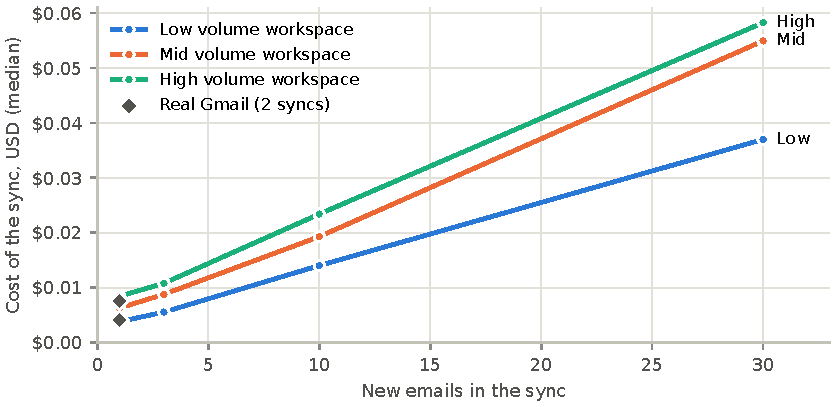
\includegraphics[width=0.86\linewidth]{figures/fig_sync_cost.pdf}
\caption{Sync cost against the number of new emails.}
\label{fig:sync}
\end{figure}

A sync has a fixed part and a part per email. The fixed part grows with the workspace, because
the guide and the current records are sent with every batch: it is \Nsyncfixedlow{} for a
low-volume workspace and \Nsyncfixedhigh{} for a high-volume one. The real Gmail syncs (1 new
email each, \usd{0.004} and \usd{0.008}) are in the same range.

The monthly cost then depends on how many new emails match the queries per day and on how they
are spread over the day. Table~\ref{tab:upkeep} assumes emails arrive at random times, so
several can land in the same 10-minute sync.

\begin{table}[H]
\centering\small
\begin{tabularx}{\linewidth}{@{}Lrrrrrrr@{}}
\toprule
& \textbf{New emails} & & \textbf{Fixed} & \textbf{Per} & \textbf{Syncs with} & \textbf{Estimate} & \\
\textbf{Volume} & \textbf{per day} & \textbf{Records} & \textbf{per sync} & \textbf{email} & \textbf{mail per day} & \textbf{per month} & \textbf{Range} \\
\midrule
\tabin{generated/tab_upkeep.tex}
\bottomrule
\end{tabularx}
\caption{Monthly cost of keeping one workspace updated. ``Fixed per sync'' and ``per email'' are
a straight-line fit to the measured syncs of that workspace size. The range runs from all of a
day's emails arriving together to every email arriving in its own sync.}
\label{tab:upkeep}
\end{table}

Three cautions on these estimates:
\begin{itemize}
\item \textbf{``New emails'' means emails matching the queries}, including promotions and other noise the agent then ignores. The queries are deliberately broad, so this number is higher than the number of emails the user cares about.
\item \textbf{The fixed part grows as the workspace fills up.} A workspace that keeps adding records for months moves towards the high-volume line, up to the 500-record limit.
\item \textbf{The 144 automatic syncs per day that find nothing are free in model cost}, but each makes one Gmail search per query.
\end{itemize}

\subsection{Other operations}

\begin{table}[H]
\centering\small
\begin{tabularx}{0.92\linewidth}{@{}Lrrrrr@{}}
\toprule
\textbf{Operation} & \textbf{n} & \textbf{Median cost} & \textbf{Range} & \textbf{Median time} & \textbf{Range} \\
\midrule
\tabin{generated/tab_other.tex}
\bottomrule
\end{tabularx}
\caption{Edits and syncs measured on the eval scenarios, with the real Gmail runs for
comparison.}
\end{table}

\subsection{Final estimates}

\begin{center}\small\renewcommand{\arraystretch}{1.35}
\begin{tabularx}{\linewidth}{@{}P{5.2cm}LLL@{}}
\toprule
& \textbf{Low volume} & \textbf{Mid volume} & \textbf{High volume} \\
\midrule
Build a workspace (one-off) & \$0.066 & \$0.14 & \$0.24 \\
Keep it updated (per month) & \$0.20 & \$1.66 & \$10.1 \\
Build time (median) & 17\,s & 18\,s & 26\,s \\
\bottomrule
\end{tabularx}\end{center}


\begin{itemize}
\item \textbf{Per user, first month}: one build plus one month of upkeep per workspace, so roughly \Nbuildlowcost{} + \Nupkeeplow{} at low volume and \Nbuildhighcost{} + \Nupkeephigh{} at high volume, before any chat edits (2 to 6 cents each in the few measured).
\item \textbf{The steady-state cost is the upkeep}, not the build. At high volume one month of syncing costs many times the build.
\item \textbf{These figures scale with the model's price.} A model that costs five times more per token costs about five times more here, and one with a thinking pass more than that. They are specific to \code{Qwen/Qwen3.8-27B} on Nebius at November 2026 list prices.
\item \textbf{The cheapest lever on upkeep} is to stop sending all records with every sync (send only the records that the new threads could match), which would remove most of the fixed part at high volume. This has not been built.
\end{itemize}
